\documentclass[10pt,a4paper]{article}\usepackage[]{graphicx}\usepackage[]{color}
%% maxwidth is the original width if it is less than linewidth
%% otherwise use linewidth (to make sure the graphics do not exceed the margin)
\makeatletter
\def\maxwidth{ %
  \ifdim\Gin@nat@width>\linewidth
    \linewidth
  \else
    \Gin@nat@width
  \fi
}
\makeatother

\definecolor{fgcolor}{rgb}{0.345, 0.345, 0.345}
\newcommand{\hlnum}[1]{\textcolor[rgb]{0.686,0.059,0.569}{#1}}%
\newcommand{\hlstr}[1]{\textcolor[rgb]{0.192,0.494,0.8}{#1}}%
\newcommand{\hlcom}[1]{\textcolor[rgb]{0.678,0.584,0.686}{\textit{#1}}}%
\newcommand{\hlopt}[1]{\textcolor[rgb]{0,0,0}{#1}}%
\newcommand{\hlstd}[1]{\textcolor[rgb]{0.345,0.345,0.345}{#1}}%
\newcommand{\hlkwa}[1]{\textcolor[rgb]{0.161,0.373,0.58}{\textbf{#1}}}%
\newcommand{\hlkwb}[1]{\textcolor[rgb]{0.69,0.353,0.396}{#1}}%
\newcommand{\hlkwc}[1]{\textcolor[rgb]{0.333,0.667,0.333}{#1}}%
\newcommand{\hlkwd}[1]{\textcolor[rgb]{0.737,0.353,0.396}{\textbf{#1}}}%

\usepackage{framed}
\makeatletter
\newenvironment{kframe}{%
 \def\at@end@of@kframe{}%
 \ifinner\ifhmode%
  \def\at@end@of@kframe{\end{minipage}}%
  \begin{minipage}{\columnwidth}%
 \fi\fi%
 \def\FrameCommand##1{\hskip\@totalleftmargin \hskip-\fboxsep
 \colorbox{shadecolor}{##1}\hskip-\fboxsep
     % There is no \\@totalrightmargin, so:
     \hskip-\linewidth \hskip-\@totalleftmargin \hskip\columnwidth}%
 \MakeFramed {\advance\hsize-\width
   \@totalleftmargin\z@ \linewidth\hsize
   \@setminipage}}%
 {\par\unskip\endMakeFramed%
 \at@end@of@kframe}
\makeatother

\definecolor{shadecolor}{rgb}{.97, .97, .97}
\definecolor{messagecolor}{rgb}{0, 0, 0}
\definecolor{warningcolor}{rgb}{1, 0, 1}
\definecolor{errorcolor}{rgb}{1, 0, 0}
\newenvironment{knitrout}{}{} % an empty environment to be redefined in TeX

\usepackage{alltt}
\usepackage[latin1]{inputenc}
\usepackage{amsmath}
\usepackage{amsfonts}
\usepackage{amssymb}
\author{Erika Martínez}
\title{Guías prácticas}
\IfFileExists{upquote.sty}{\usepackage{upquote}}{}
\begin{document}

\maketitle
\newpage

UNIDAD 2: Pr?ctica 08 AN?LISIS ESTAD?STICO DE LOS DATOS. 
Crea el vector que contendr? los datos. 
\begin{knitrout}
\definecolor{shadecolor}{rgb}{0.969, 0.969, 0.969}\color{fgcolor}\begin{kframe}
\begin{alltt}
\hlstd{Notas} \hlkwb{<-} \hlkwd{c}\hlstd{(}\hlnum{4.47}\hlstd{,} \hlnum{5.43}\hlstd{); Notas}
\end{alltt}
\begin{verbatim}
## [1] 4.47 5.43
\end{verbatim}
\begin{alltt}
\hlkwd{data.entry}\hlstd{(Notas)}
\hlstd{Notas}
\end{alltt}
\begin{verbatim}
## [1] 4.47 5.43
\end{verbatim}
\begin{alltt}
\hlkwd{length}\hlstd{(Notas)}
\end{alltt}
\begin{verbatim}
## [1] 2
\end{verbatim}
\end{kframe}
\end{knitrout}

Guarda el vector de datos en un archivo. 
\begin{knitrout}
\definecolor{shadecolor}{rgb}{0.969, 0.969, 0.969}\color{fgcolor}\begin{kframe}
\begin{alltt}
\hlkwd{write}\hlstd{(Notas,} \hlstr{"Notas.txt"}\hlstd{)}
\end{alltt}
\end{kframe}
\end{knitrout}

Lee o recupera el vector de datos desde el archivo de texto. 
\begin{knitrout}
\definecolor{shadecolor}{rgb}{0.969, 0.969, 0.969}\color{fgcolor}\begin{kframe}
\begin{alltt}
\hlstd{X} \hlkwb{<-} \hlkwd{scan}\hlstd{(}\hlstr{"Notas.txt"}\hlstd{,} \hlkwc{what} \hlstd{=} \hlkwd{double}\hlstd{(}\hlnum{0}\hlstd{),} \hlkwc{na.strings} \hlstd{=} \hlstr{"NA"}\hlstd{,} \hlkwc{flush}\hlstd{=}\hlnum{FALSE}\hlstd{)}
\hlkwd{ls}\hlstd{()}
\end{alltt}
\begin{verbatim}
## [1] "Notas" "X"
\end{verbatim}
\end{kframe}
\end{knitrout}



Crea la tabla de frecuencias. 
Usa el M?todo de Herbert A. Sturges para determinar dicho n?mero. 
\begin{knitrout}
\definecolor{shadecolor}{rgb}{0.969, 0.969, 0.969}\color{fgcolor}\begin{kframe}
\begin{alltt}
\hlstd{n} \hlkwb{<-} \hlkwd{length}\hlstd{(X); n}
\end{alltt}
\begin{verbatim}
## [1] 2
\end{verbatim}
\begin{alltt}
\hlstd{k} \hlkwb{<-} \hlnum{1}\hlopt{+}\hlnum{3.322}\hlopt{*}\hlkwd{logb}\hlstd{(n,} \hlnum{10}\hlstd{); k}
\end{alltt}
\begin{verbatim}
## [1] 2.000022
\end{verbatim}
\begin{alltt}
\hlstd{k} \hlkwb{<-} \hlkwd{round}\hlstd{(k); k}
\end{alltt}
\begin{verbatim}
## [1] 2
\end{verbatim}
\end{kframe}
\end{knitrout}

Calcula el ancho o amplitud a de cada intervalo a=rango/k 
\begin{knitrout}
\definecolor{shadecolor}{rgb}{0.969, 0.969, 0.969}\color{fgcolor}\begin{kframe}
\begin{alltt}
\hlstd{rango} \hlkwb{<-} \hlkwd{max}\hlstd{(X)}\hlopt{-}\hlkwd{min}\hlstd{(X); rango}
\end{alltt}
\begin{verbatim}
## [1] 0.96
\end{verbatim}
\begin{alltt}
\hlstd{a}\hlkwb{=}\hlstd{rango}\hlopt{/}\hlstd{k; a}
\end{alltt}
\begin{verbatim}
## [1] 0.48
\end{verbatim}
\begin{alltt}
\hlstd{a} \hlkwb{<-} \hlkwd{round}\hlstd{(a,} \hlnum{3}\hlstd{); a}
\end{alltt}
\begin{verbatim}
## [1] 0.48
\end{verbatim}
\end{kframe}
\end{knitrout}

 Define los l?mites y puntos mediosde cada uno de los k intervalos 
\begin{knitrout}
\definecolor{shadecolor}{rgb}{0.969, 0.969, 0.969}\color{fgcolor}\begin{kframe}
\begin{alltt}
\hlstd{limites} \hlkwb{<-} \hlkwd{seq}\hlstd{(}\hlkwc{from}\hlstd{=}\hlkwd{min}\hlstd{(X)}\hlopt{-}\hlnum{0.01}\hlopt{/}\hlnum{2}\hlstd{,}\hlkwc{to}\hlstd{=}\hlkwd{max}\hlstd{(X)}\hlopt{+}\hlnum{0.01}\hlopt{/}\hlnum{2}\hlstd{,} \hlkwc{by}\hlstd{=a); limites}
\end{alltt}
\begin{verbatim}
## [1] 4.465 4.945 5.425
\end{verbatim}
\begin{alltt}
\hlkwd{options}\hlstd{(}\hlkwc{digits}\hlstd{=}\hlnum{4}\hlstd{)}
\hlstd{ci} \hlkwb{<-} \hlkwd{cbind}\hlstd{(}\hlnum{1}\hlopt{:}\hlstd{k); ci}
\end{alltt}
\begin{verbatim}
##      [,1]
## [1,]    1
## [2,]    2
\end{verbatim}
\begin{alltt}
\hlkwa{for}\hlstd{(i} \hlkwa{in} \hlnum{2}\hlopt{:}\hlkwd{length}\hlstd{(limites)) ci[i}\hlopt{-}\hlnum{1}\hlstd{,} \hlnum{1}\hlstd{]} \hlkwb{<-} \hlstd{(limites[i]} \hlopt{+} \hlstd{limites[i}\hlopt{-}\hlnum{1}\hlstd{])}\hlopt{/}\hlnum{2}
\hlstd{ci}
\end{alltt}
\begin{verbatim}
##       [,1]
## [1,] 4.705
## [2,] 5.185
\end{verbatim}
\end{kframe}
\end{knitrout}

 Encuentra las frecuencias absolutas fi para cada intervalo. 
\begin{knitrout}
\definecolor{shadecolor}{rgb}{0.969, 0.969, 0.969}\color{fgcolor}\begin{kframe}
\begin{alltt}
\hlkwd{options}\hlstd{(}\hlkwc{digits}\hlstd{=}\hlnum{2}\hlstd{)}
\hlstd{fi} \hlkwb{<-} \hlkwd{cbind}\hlstd{(}\hlkwd{table}\hlstd{(}\hlkwd{cut}\hlstd{(Notas,} \hlkwc{breaks} \hlstd{= limites,} \hlkwc{labels}\hlstd{=}\hlkwa{NULL}\hlstd{,} \hlkwc{include.lowest}\hlstd{=}\hlnum{FALSE}\hlstd{,}
\hlkwc{right}\hlstd{=}\hlnum{FALSE}\hlstd{,} \hlkwc{dig.lab}\hlstd{=}\hlnum{4}\hlstd{))); fi}
\end{alltt}
\begin{verbatim}
##               [,1]
## [4.465,4.945)    1
## [4.945,5.425)    0
\end{verbatim}
\end{kframe}
\end{knitrout}

Encuentra las frecuencias relativas o proporciones fri. 
\begin{knitrout}
\definecolor{shadecolor}{rgb}{0.969, 0.969, 0.969}\color{fgcolor}\begin{kframe}
\begin{alltt}
\hlkwd{options}\hlstd{(}\hlkwc{digits}\hlstd{=}\hlnum{4}\hlstd{)}
\hlstd{fri} \hlkwb{<-} \hlstd{fi}\hlopt{/}\hlstd{n; fri}
\end{alltt}
\begin{verbatim}
##               [,1]
## [4.465,4.945)  0.5
## [4.945,5.425)  0.0
\end{verbatim}
\end{kframe}
\end{knitrout}

Encuentra las frecuencias acumuladas ascendentes Fi 
\begin{knitrout}
\definecolor{shadecolor}{rgb}{0.969, 0.969, 0.969}\color{fgcolor}\begin{kframe}
\begin{alltt}
\hlkwd{options}\hlstd{(}\hlkwc{digits}\hlstd{=}\hlnum{2}\hlstd{)}
\hlstd{Fi} \hlkwb{<-} \hlkwd{cumsum}\hlstd{(fi); Fi}
\end{alltt}
\begin{verbatim}
## [1] 1 1
\end{verbatim}
\end{kframe}
\end{knitrout}

 Encuentra las frecuencias relativas acumuladas Fri 
\begin{knitrout}
\definecolor{shadecolor}{rgb}{0.969, 0.969, 0.969}\color{fgcolor}\begin{kframe}
\begin{alltt}
\hlkwd{options}\hlstd{(}\hlkwc{digits}\hlstd{=}\hlnum{4}\hlstd{)}
\hlstd{Fri} \hlkwb{<-} \hlstd{Fi}\hlopt{/}\hlstd{n; Fri}
\end{alltt}
\begin{verbatim}
## [1] 0.5 0.5
\end{verbatim}
\end{kframe}
\end{knitrout}

Completa la tabla de frecuencias. 
\begin{knitrout}
\definecolor{shadecolor}{rgb}{0.969, 0.969, 0.969}\color{fgcolor}\begin{kframe}
\begin{alltt}
\hlstd{tablaFrec} \hlkwb{<-} \hlkwd{data.frame}\hlstd{(}\hlkwc{ci}\hlstd{=ci,} \hlkwc{fi}\hlstd{=fi,} \hlkwc{fri}\hlstd{=fri,} \hlkwc{Fi}\hlstd{=Fi,} \hlkwc{Fri}\hlstd{=Fri); tablaFrec}
\end{alltt}
\begin{verbatim}
##                  ci fi fri Fi Fri
## [4.465,4.945) 4.705  1 0.5  1 0.5
## [4.945,5.425) 5.185  0 0.0  1 0.5
\end{verbatim}
\end{kframe}
\end{knitrout}

Crea el histograma de frecuencias 
\begin{knitrout}
\definecolor{shadecolor}{rgb}{0.969, 0.969, 0.969}\color{fgcolor}\begin{kframe}
\begin{alltt}
\hlstd{h} \hlkwb{<-} \hlkwd{hist}\hlstd{(X,} \hlkwc{breaks}\hlstd{=}\hlkwd{c}\hlstd{(limites[}\hlnum{1}\hlstd{]}\hlopt{-}\hlstd{a, limites, limites[k}\hlopt{+}\hlnum{1}\hlstd{]}\hlopt{+}\hlstd{a),} \hlkwc{freq} \hlstd{=} \hlnum{TRUE}\hlstd{,} \hlkwc{probability} \hlstd{=} \hlnum{FALSE}\hlstd{,}
\hlkwc{include.lowest} \hlstd{=} \hlnum{FALSE}\hlstd{,}\hlkwc{right} \hlstd{=} \hlnum{TRUE}\hlstd{,} \hlkwc{main} \hlstd{=} \hlstr{"Histograma de frecuencias"}\hlstd{,}
\hlkwc{col}\hlstd{=}\hlstr{"lightyellow"}\hlstd{,} \hlkwc{lty}\hlstd{=}\hlnum{1}\hlstd{,} \hlkwc{border}\hlstd{=}\hlstr{"purple"}\hlstd{,} \hlkwc{xlab}\hlstd{=}\hlstr{"Notas de aspirantes"}\hlstd{,} \hlkwc{ylab}\hlstd{=}\hlstr{"Frecuencia (fi)"}\hlstd{,}
\hlkwc{axes}\hlstd{=}\hlnum{TRUE}\hlstd{,} \hlkwc{labels}\hlstd{=}\hlnum{FALSE}\hlstd{)}
\hlkwd{text}\hlstd{(h}\hlopt{$}\hlstd{mids, h}\hlopt{$}\hlstd{density, h}\hlopt{$}\hlstd{counts,} \hlkwc{adj}\hlstd{=}\hlkwd{c}\hlstd{(}\hlnum{0.5}\hlstd{,} \hlopt{-}\hlnum{0.5}\hlstd{),} \hlkwc{col}\hlstd{=}\hlstr{"red"}\hlstd{)}
\hlkwd{rug}\hlstd{(}\hlkwd{jitter}\hlstd{(Notas))}
\end{alltt}
\end{kframe}
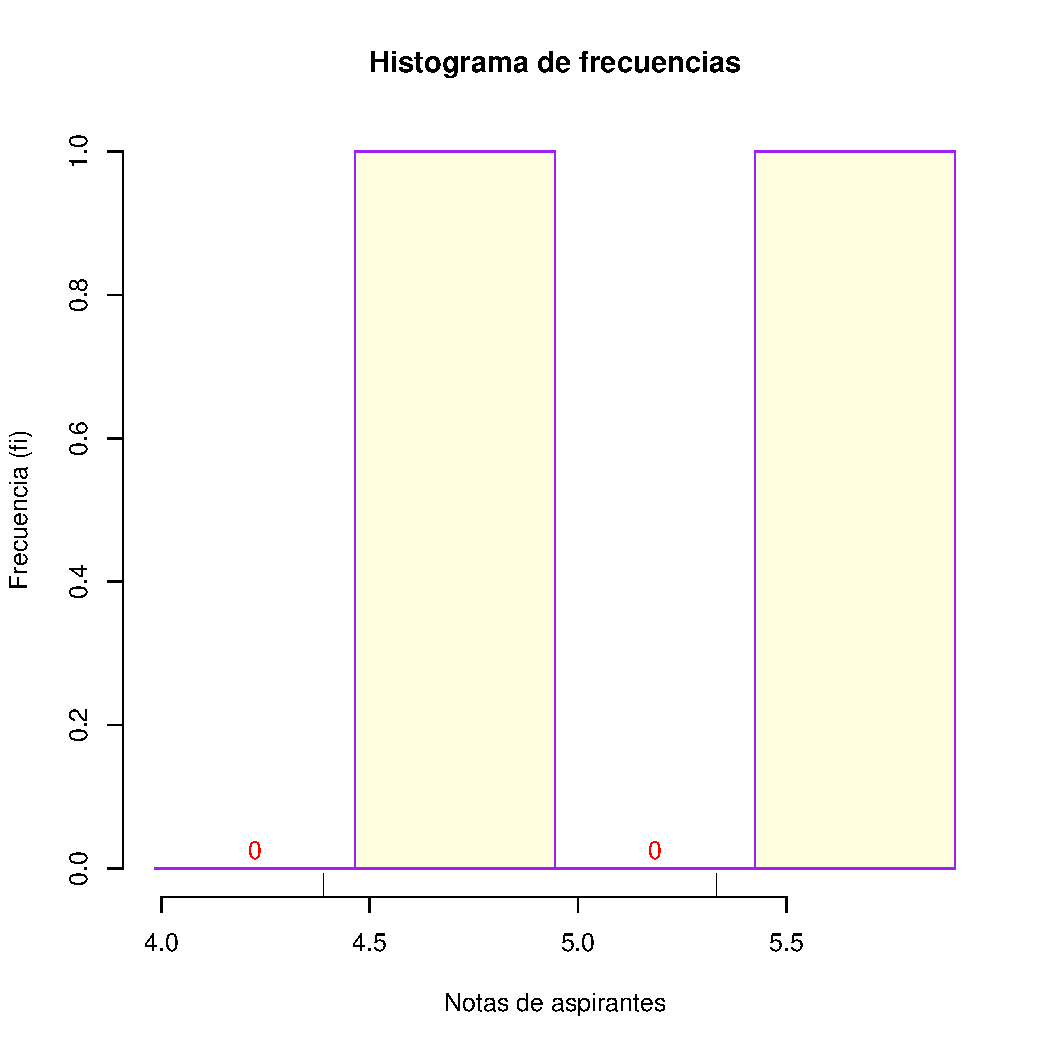
\includegraphics[width=\maxwidth]{figure/unnamed-chunk-12-1} 
\begin{kframe}\begin{alltt}
\hlkwd{is.list}\hlstd{(h); h}
\end{alltt}
\begin{verbatim}
## [1] TRUE
## $breaks
## [1] 3.985 4.465 4.945 5.425 5.905
## 
## $counts
## [1] 0 1 0 1
## 
## $density
## [1] 0.000 1.042 0.000 1.042
## 
## $mids
## [1] 4.225 4.705 5.185 5.665
## 
## $xname
## [1] "X"
## 
## $equidist
## [1] TRUE
## 
## attr(,"class")
## [1] "histogram"
\end{verbatim}
\end{kframe}
\end{knitrout}

Aproxima al histograma la funci?n de densidad normal 
\begin{knitrout}
\definecolor{shadecolor}{rgb}{0.969, 0.969, 0.969}\color{fgcolor}\begin{kframe}
\begin{alltt}
\hlstd{h} \hlkwb{<-} \hlkwd{hist}\hlstd{(X,} \hlkwc{breaks}\hlstd{=}\hlkwd{c}\hlstd{(limites[}\hlnum{1}\hlstd{]}\hlopt{-}\hlstd{a, limites, limites[k}\hlopt{+}\hlnum{1}\hlstd{]}\hlopt{+}\hlstd{a),} \hlkwc{freq} \hlstd{=} \hlnum{FALSE}\hlstd{,}
\hlkwc{probability} \hlstd{=} \hlnum{TRUE}\hlstd{,} \hlkwc{include.lowest} \hlstd{=} \hlnum{FALSE}\hlstd{,} \hlkwc{right} \hlstd{=} \hlnum{TRUE}\hlstd{,}
\hlkwc{main}\hlstd{=}\hlstr{"Aproximaci?n a una Normal\textbackslash{}n"}\hlstd{,} \hlkwc{col}\hlstd{=}\hlstr{"lightyellow"}\hlstd{,}\hlkwc{lty}\hlstd{=}\hlnum{1}\hlstd{,}\hlkwc{border}\hlstd{=}\hlstr{"purple"}\hlstd{,}
\hlkwc{xlab}\hlstd{=}\hlstr{"Notas de aspirantes\textbackslash{}n"}\hlstd{,} \hlkwc{ylab}\hlstd{=}\hlstr{"Frecuencia relativa (fri)"}\hlstd{,}
\hlkwc{axes}\hlstd{=}\hlnum{TRUE}\hlstd{,} \hlkwc{labels}\hlstd{=}\hlnum{FALSE}\hlstd{)}
\hlkwd{text}\hlstd{(h}\hlopt{$}\hlstd{mids, h}\hlopt{$}\hlstd{density, h}\hlopt{$}\hlstd{counts,} \hlkwc{adj}\hlstd{=}\hlkwd{c}\hlstd{(}\hlnum{0.5}\hlstd{,} \hlnum{0.2}\hlstd{),} \hlkwc{col}\hlstd{=}\hlstr{"red"}\hlstd{)}
\hlkwd{rug}\hlstd{(}\hlkwd{jitter}\hlstd{(X))} \hlcom{# adiciona marcas de los datos }
\hlkwd{curve}\hlstd{(}\hlkwd{dnorm}\hlstd{(x,} \hlkwc{mean}\hlstd{=}\hlkwd{mean}\hlstd{(X),} \hlkwc{sd}\hlstd{=}\hlkwd{sd}\hlstd{(X)),} \hlkwc{col} \hlstd{=} \hlnum{2}\hlstd{,} \hlkwc{lty} \hlstd{=} \hlnum{2}\hlstd{,}\hlkwc{lwd} \hlstd{=} \hlnum{2}\hlstd{,} \hlkwc{add} \hlstd{=} \hlnum{TRUE}\hlstd{)}
\end{alltt}
\end{kframe}
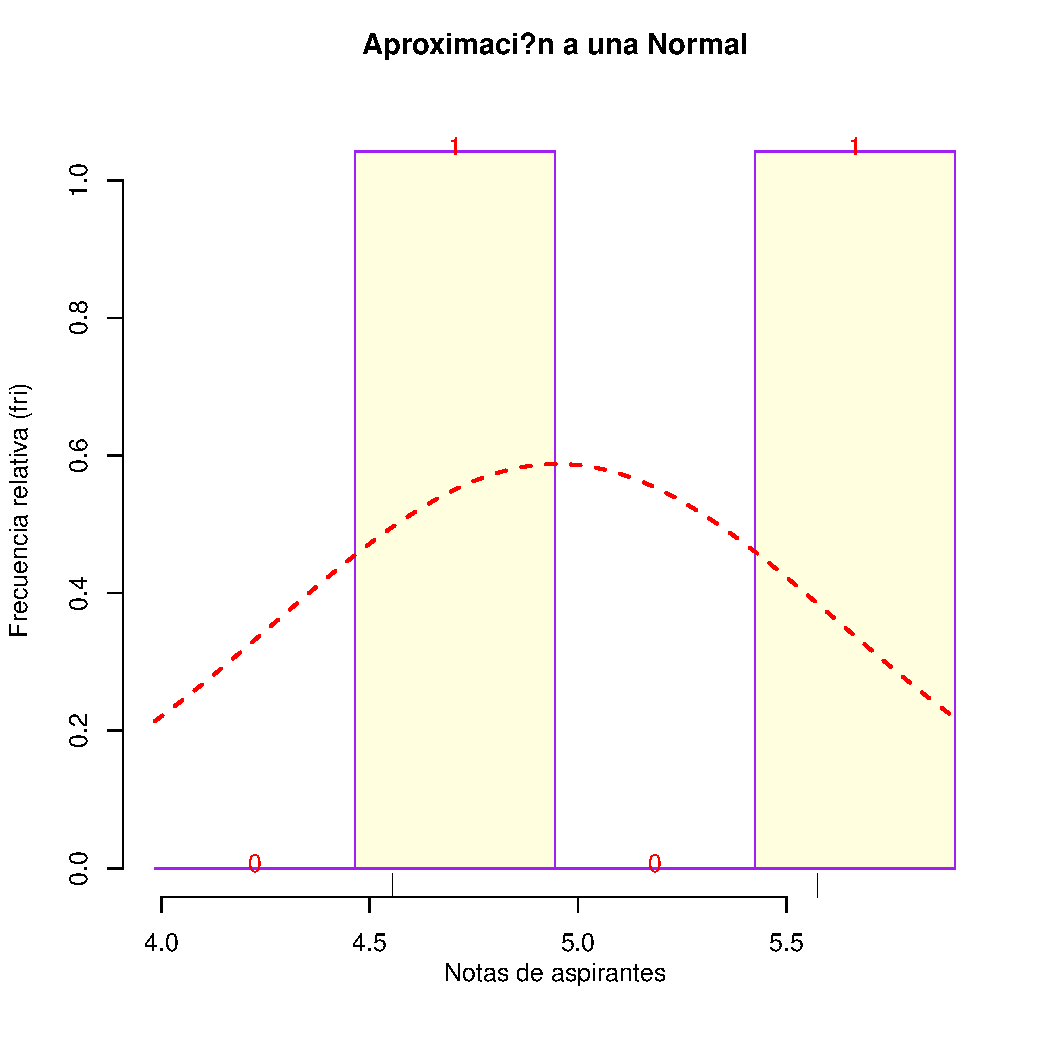
\includegraphics[width=\maxwidth]{figure/unnamed-chunk-13-1} 

\end{knitrout}

Crea el pol?gono de frecuencias 
\begin{knitrout}
\definecolor{shadecolor}{rgb}{0.969, 0.969, 0.969}\color{fgcolor}\begin{kframe}
\begin{alltt}
\hlstd{h} \hlkwb{<-} \hlkwd{hist}\hlstd{(X,} \hlkwc{breaks}\hlstd{=}\hlkwd{c}\hlstd{(limites[}\hlnum{1}\hlstd{]}\hlopt{-}\hlstd{a, limites, limites[k}\hlopt{+}\hlnum{1}\hlstd{]}\hlopt{+}\hlstd{a),} \hlkwc{freq} \hlstd{=} \hlnum{TRUE}\hlstd{,}
\hlkwc{probability}\hlstd{=}\hlnum{FALSE}\hlstd{,} \hlkwc{include.lowest}\hlstd{=}\hlnum{FALSE}\hlstd{,}\hlkwc{right}\hlstd{=}\hlnum{TRUE}\hlstd{,}
\hlkwc{main} \hlstd{=} \hlstr{"Pol?gono de frecuencias"}\hlstd{,}\hlkwc{col}\hlstd{=}\hlstr{"lightyellow"}\hlstd{,} \hlkwc{lty}\hlstd{=}\hlnum{1}\hlstd{,} \hlkwc{border}\hlstd{=}\hlstr{"purple"}\hlstd{,} \hlkwc{xlab}\hlstd{=}\hlstr{" 
Notas de aspirantes"}\hlstd{,} \hlkwc{ylab}\hlstd{=}\hlstr{"Frecuencia (fi)"}\hlstd{,} \hlkwc{axes}\hlstd{=}\hlnum{TRUE}\hlstd{,} \hlkwc{labels}\hlstd{=}\hlnum{FALSE}\hlstd{)}
\hlkwd{text}\hlstd{(h}\hlopt{$}\hlstd{mids, h}\hlopt{$}\hlstd{density, h}\hlopt{$}\hlstd{counts,} \hlkwc{adj}\hlstd{=}\hlkwd{c}\hlstd{(}\hlnum{0.5}\hlstd{,} \hlopt{-}\hlnum{0.5}\hlstd{),} \hlkwc{col}\hlstd{=}\hlstr{"red"}\hlstd{)}
\hlkwd{rug}\hlstd{(}\hlkwd{jitter}\hlstd{(X))} \hlcom{# adiciona marcas de los datos }
\hlstd{vCi} \hlkwb{<-} \hlkwd{c}\hlstd{(h}\hlopt{$}\hlstd{mids[}\hlnum{1}\hlstd{]}\hlopt{-}\hlstd{a, h}\hlopt{$}\hlstd{mids, h}\hlopt{$}\hlstd{mids[k}\hlopt{+}\hlnum{1}\hlstd{]}\hlopt{+}\hlstd{a); vCi}
\end{alltt}
\begin{verbatim}
## [1] 3.745 4.225 4.705 5.185 5.665 5.665
\end{verbatim}
\begin{alltt}
\hlstd{vfi} \hlkwb{<-} \hlkwd{c}\hlstd{(}\hlnum{0}\hlstd{, h}\hlopt{$}\hlstd{counts,} \hlnum{0}\hlstd{); vfi}
\end{alltt}
\begin{verbatim}
## [1] 0 0 1 0 1 0
\end{verbatim}
\begin{alltt}
\hlkwd{lines}\hlstd{(vCi, vfi,} \hlkwc{col}\hlstd{=}\hlstr{"blue"}\hlstd{,} \hlkwc{type}\hlstd{=}\hlstr{"l"}\hlstd{)}
\end{alltt}
\end{kframe}
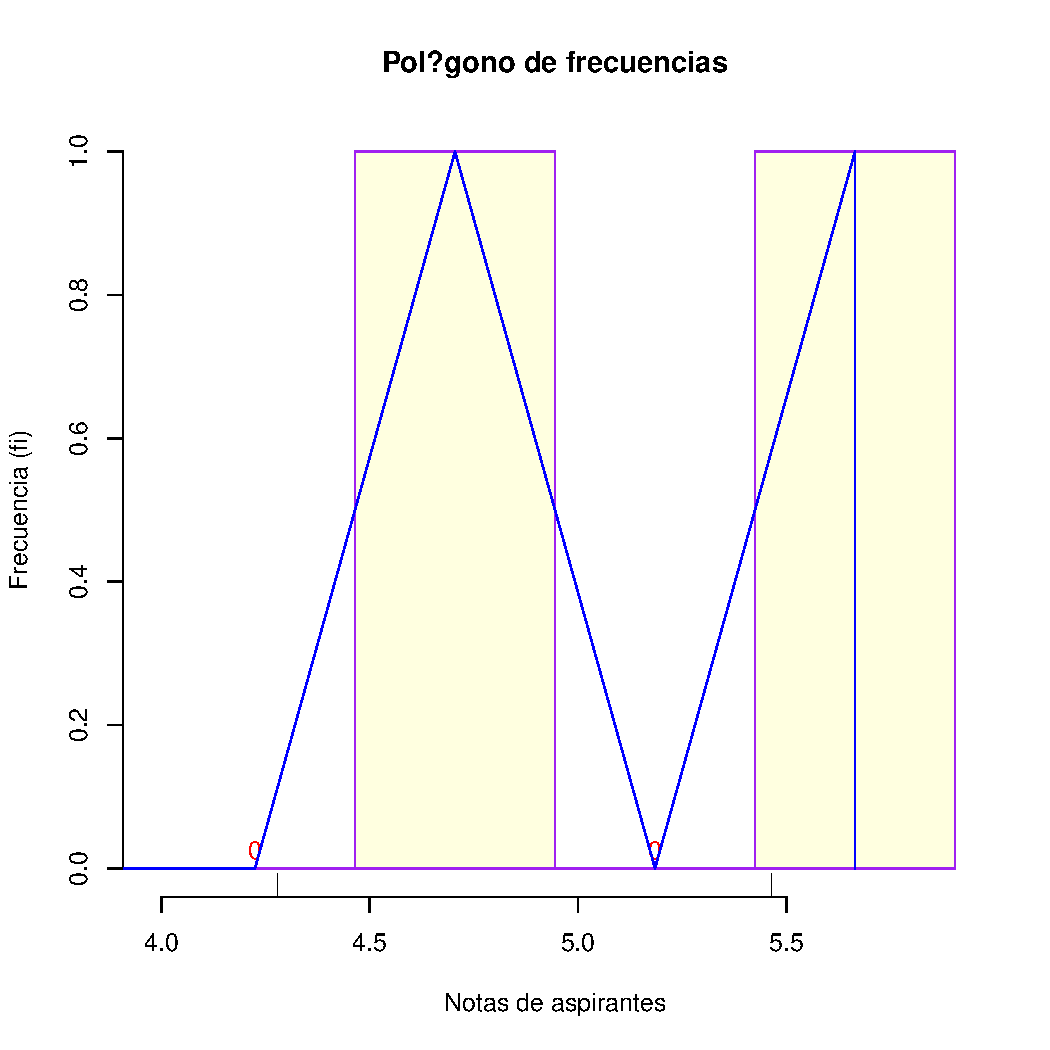
\includegraphics[width=\maxwidth]{figure/unnamed-chunk-14-1} 

\end{knitrout}

Crea la Ojiva ascendente o pol?gono de frecuencias acumuladas ascendentes 
\begin{knitrout}
\definecolor{shadecolor}{rgb}{0.969, 0.969, 0.969}\color{fgcolor}\begin{kframe}
\begin{alltt}
\hlstd{Fia} \hlkwb{<-} \hlkwd{c}\hlstd{(}\hlnum{0}\hlstd{, Fi); Fia}
\end{alltt}
\begin{verbatim}
## [1] 0 1 1
\end{verbatim}
\begin{alltt}
\hlkwd{plot}\hlstd{(limites, Fia,} \hlkwc{type} \hlstd{=} \hlstr{"p"}\hlstd{,} \hlkwc{pch}\hlstd{=}\hlnum{1}\hlstd{,} \hlkwc{col} \hlstd{=} \hlstr{"blue"}\hlstd{,} \hlkwc{main}\hlstd{=}\hlstr{"Ojiva ascendente"}\hlstd{,}
\hlkwc{xlab}\hlstd{=}\hlstr{"Notas de aspirantes"}\hlstd{,}\hlkwc{ylab}\hlstd{=}\hlstr{"Frecuencia acumulada (Fi)"}\hlstd{)}
\hlkwd{text}\hlstd{(limites, h}\hlopt{$}\hlstd{density, Fia,} \hlkwc{adj}\hlstd{=}\hlkwd{c}\hlstd{(}\hlnum{0.5}\hlstd{,} \hlopt{-}\hlnum{0.5}\hlstd{),} \hlkwc{col}\hlstd{=}\hlstr{"red"}\hlstd{)}
\hlkwd{lines}\hlstd{(limites, Fia,} \hlkwc{col}\hlstd{=}\hlstr{"black"}\hlstd{,} \hlkwc{type}\hlstd{=}\hlstr{"l"}\hlstd{)}
\end{alltt}
\end{kframe}
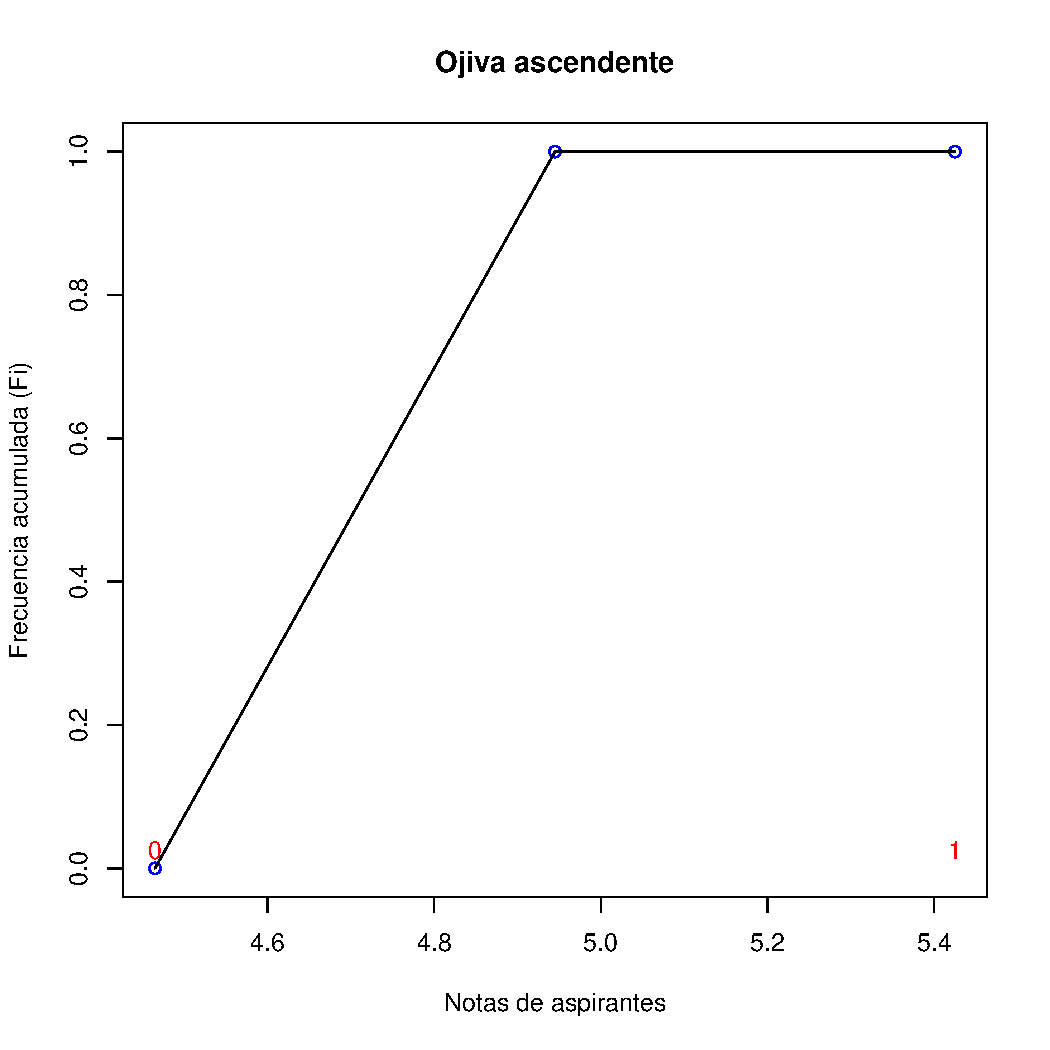
\includegraphics[width=\maxwidth]{figure/unnamed-chunk-15-1} 

\end{knitrout}

Calcula los principales estad?sticos descriptivos de la variable 
Calcula la moda, ya que el R no proporciona una funci?n para eso. 
\begin{knitrout}
\definecolor{shadecolor}{rgb}{0.969, 0.969, 0.969}\color{fgcolor}\begin{kframe}
\begin{alltt}
\hlkwd{options}\hlstd{(}\hlkwc{digits}\hlstd{=}\hlnum{4}\hlstd{)}
\hlkwa{for}\hlstd{(i} \hlkwa{in} \hlnum{1}\hlopt{:}\hlstd{k)} \hlkwa{if} \hlstd{(fi[i]} \hlopt{==} \hlkwd{max}\hlstd{(fi))} \hlkwa{break}\hlstd{()}

\hlkwa{if}\hlstd{(i} \hlopt{>} \hlnum{1}\hlstd{) moda} \hlkwb{<-} \hlstd{limites[i]}\hlopt{+}\hlstd{((fi[i]}\hlopt{-}\hlstd{fi[i}\hlopt{-}\hlnum{1}\hlstd{])}\hlopt{/}\hlstd{((fi[i]}\hlopt{-}\hlstd{fi[i}\hlopt{-}\hlnum{1}\hlstd{])}\hlopt{+}\hlstd{(fi[i]}\hlopt{-}\hlstd{fi[i}\hlopt{+}\hlnum{1}\hlstd{]) ))}\hlopt{*}\hlstd{a} \hlkwa{else} \hlstd{\{}
\hlstd{moda} \hlkwb{<-} \hlstd{limites[i]}\hlopt{+}\hlstd{(fi[i]}\hlopt{/}\hlstd{(fi[i]}\hlopt{+}\hlstd{(fi[i]}\hlopt{-}\hlstd{fi[i}\hlopt{+}\hlnum{1}\hlstd{])))}\hlopt{*}\hlstd{a}
\hlstd{moda \}}
\end{alltt}
\begin{verbatim}
## [1] 4.705
\end{verbatim}
\end{kframe}
\end{knitrout}

 Calcula los cuartiles: Q1, Q2, Q3 
\begin{knitrout}
\definecolor{shadecolor}{rgb}{0.969, 0.969, 0.969}\color{fgcolor}\begin{kframe}
\begin{alltt}
\hlstd{Q} \hlkwb{<-} \hlnum{1}\hlopt{:}\hlnum{3}
\hlkwa{for}\hlstd{(v} \hlkwa{in} \hlnum{1}\hlopt{:}\hlnum{3}\hlstd{)} \hlkwa{for}\hlstd{(i} \hlkwa{in} \hlnum{1}\hlopt{:}\hlstd{k)} \hlkwa{if} \hlstd{(Fi[i]} \hlopt{>} \hlstd{(v}\hlopt{*}\hlnum{25}\hlopt{*}\hlstd{n)}\hlopt{/}\hlnum{100}\hlstd{)}
\hlstd{\{}
  \hlstd{Q[v]} \hlkwb{<-} \hlstd{limites[i]}\hlopt{+}\hlstd{(((}\hlnum{25}\hlopt{*}\hlstd{v}\hlopt{*}\hlstd{n}\hlopt{/}\hlnum{100}\hlstd{)}\hlopt{-}\hlstd{Fi[i}\hlopt{-}\hlnum{1}\hlstd{])}\hlopt{/}\hlstd{fi[i])}\hlopt{*}\hlstd{a}
  \hlkwa{break}
\hlstd{\}}
\end{alltt}


{\ttfamily\noindent\bfseries\color{errorcolor}{\#\# Error in Q[v] <- limites[i] + (((25 * v * n/100) - Fi[i - 1])/fi[i]) * : replacement has length zero}}\begin{alltt}
\hlstd{Q}
\end{alltt}
\begin{verbatim}
## [1] 1 2 3
\end{verbatim}
\end{kframe}
\end{knitrout}


Calcula los principales estad?sticos. 
\begin{knitrout}
\definecolor{shadecolor}{rgb}{0.969, 0.969, 0.969}\color{fgcolor}\begin{kframe}
\begin{alltt}
\hlstd{estadisticos} \hlkwb{<-} \hlkwd{rbind}\hlstd{(}\hlkwc{media}\hlstd{=}\hlkwd{sum}\hlstd{(tabEstad}\hlopt{$}\hlstd{cifi)}\hlopt{/}\hlstd{n,} \hlkwc{moda}\hlstd{=moda,} \hlkwc{Q1}\hlstd{=Q[}\hlnum{1}\hlstd{],} \hlkwc{Q2}\hlstd{=Q[}\hlnum{2}\hlstd{],} \hlkwc{Q3}\hlstd{=Q[}\hlnum{3}\hlstd{],}
\hlkwc{rango}\hlstd{=}\hlkwd{max}\hlstd{(X)}\hlopt{-}\hlkwd{min}\hlstd{(X),}  \hlkwc{varianza}\hlstd{=}\hlkwd{sum}\hlstd{(tabEstad}\hlopt{$}\hlstd{ciMedia2fi)}\hlopt{/}\hlstd{n,}
\hlkwc{Desviacion}\hlstd{=}\hlkwd{sqrt}\hlstd{(}\hlkwd{sum}\hlstd{(tabEstad}\hlopt{$}\hlstd{ciMedia2fi)}\hlopt{/}\hlstd{n),}
\hlkwc{CoeficienteVariacion}\hlstd{=}\hlkwd{sqrt}\hlstd{(}\hlkwd{sum}\hlstd{(tabEstad}\hlopt{$}\hlstd{ciMedia2fi)}\hlopt{/}\hlstd{n)}\hlopt{/}\hlstd{(}\hlkwd{sum}\hlstd{(tabEstad}\hlopt{$}\hlstd{cifi)}\hlopt{/}\hlstd{n),}
\hlkwc{CAfisher}\hlstd{=(}\hlkwd{sum}\hlstd{(tabEstad}\hlopt{$}\hlstd{ciMedia3fi)}\hlopt{/}\hlstd{n)}\hlopt{/}\hlkwd{sqrt}\hlstd{(}\hlkwd{sum}\hlstd{(tabEstad}\hlopt{$}\hlstd{ciMedia2fi)}\hlopt{/}\hlstd{n)}\hlopt{^}\hlnum{3}\hlstd{,}
\hlkwc{CoeficienteCurtosis}\hlstd{=((}\hlkwd{sum}\hlstd{(tabEstad}\hlopt{$}\hlstd{ciMedia4fi)}\hlopt{/}\hlstd{n)}\hlopt{/}\hlkwd{sqrt}\hlstd{(}\hlkwd{sum}\hlstd{(tabEstad}\hlopt{$}\hlstd{ciMedia2fi)}\hlopt{/}\hlstd{n)}\hlopt{^}\hlnum{4}\hlstd{)}\hlopt{-}\hlnum{3}\hlstd{)}
\end{alltt}


{\ttfamily\noindent\bfseries\color{errorcolor}{\#\# Error in rbind(media = sum(tabEstad\$cifi)/n, moda = moda, Q1 = Q[1], Q2 = Q[2], : objeto 'tabEstad' no encontrado}}\begin{alltt}
\hlstd{estadisticos}
\end{alltt}


{\ttfamily\noindent\bfseries\color{errorcolor}{\#\# Error in eval(expr, envir, enclos): objeto 'estadisticos' no encontrado}}\end{kframe}
\end{knitrout}

Otros gr?ficos: 
Gr?fico de cajas 
\begin{knitrout}
\definecolor{shadecolor}{rgb}{0.969, 0.969, 0.969}\color{fgcolor}\begin{kframe}
\begin{alltt}
\hlkwd{boxplot}\hlstd{(}\hlnum{2}\hlstd{,} \hlkwc{main}\hlstd{=}\hlstr{"Gr?fico de caja"}\hlstd{,} \hlkwc{xlab}\hlstd{=}\hlstr{"Notas"}\hlstd{,} \hlkwc{notch}\hlstd{=}\hlnum{FALSE}\hlstd{,}
\hlkwc{data}\hlstd{=}\hlkwd{parent.frame}\hlstd{(),} \hlkwc{plot}\hlstd{=}\hlnum{TRUE}\hlstd{,} \hlkwc{border}\hlstd{=}\hlstr{"red"}\hlstd{,} \hlkwc{col}\hlstd{=}\hlstr{"yellow"}\hlstd{,}\hlkwc{horizontal}\hlstd{=}\hlnum{TRUE}\hlstd{)}
\end{alltt}
\end{kframe}
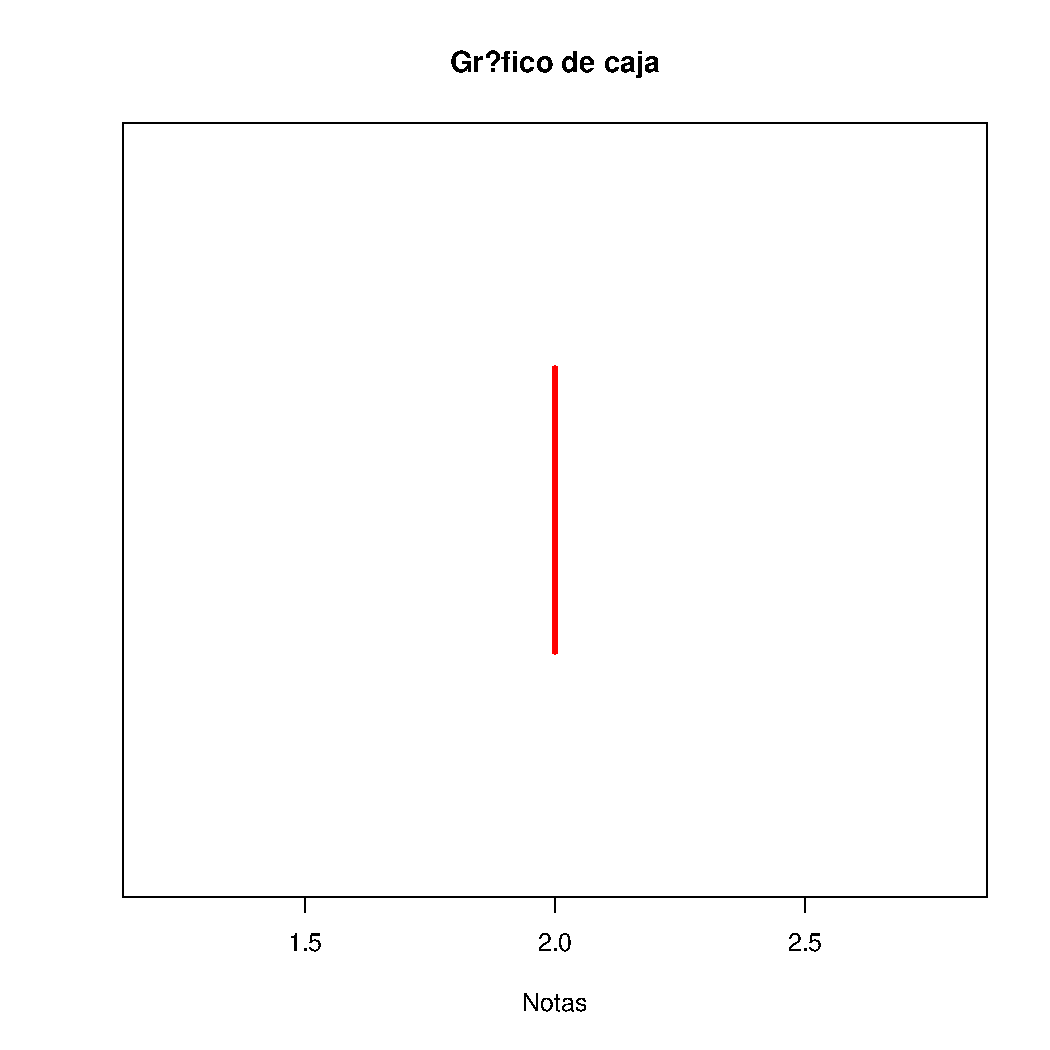
\includegraphics[width=\maxwidth]{figure/unnamed-chunk-19-1} 

\end{knitrout}



\end{document}
